\documentclass{article}
\usepackage[utf8]{inputenc}

\title{Título}
\author{Autor: Oscar Yantza}
\date{October 2019}

\usepackage{natbib}
\usepackage{graphicx}

\begin{document}

\maketitle

\section{Introduccción}
There is a theory which states that if ever anyone discovers exactly what the Universe is for and why it is here, it will instantly disappear and be replaced by something even more bizarre and inexplicable.\n

APECTOS A TOMAR EN CUENTA:
\begin{enumerate}
    \item ¿El ensayo tiene un buen párrafo de apertura / introducción?
    \item ¿Está claro el tema?
    \item ¿Se sabe cuál es la intención?
\end{enumerate}
$\sigma^{2}=\frac{\sum(x-\bar{x})^{2}}{N}$

\begin{figure}[h!]
\centering
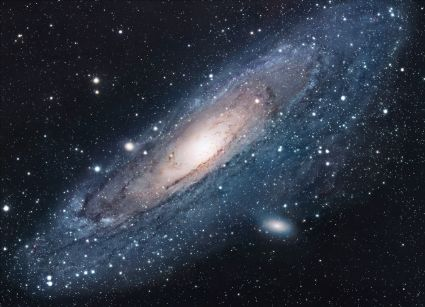
\includegraphics[scale=1.7]{universe}
\caption{The Universe}
\label{fig:universe}
\end{figure}


\section{Desarrollo}

There is a theory which states that if ever anyone discovers exactly what the Universe is for and why it is here, it will instantly disappear and be replaced by something even more bizarre and inexplicable.\n
NO SE OLVIDE DE CITAR DE FORMA CORRECTA USE MENDELEY PARA ESTE APARTADO, RECUERDE USAR IEEE

``I always thought something was fundamentally wrong with the universe'' \citep{adams1995hitchhiker}

ASPECTOS A TOMAR EN CUENTA:

\begin{itemize}
    \item  ¿Está el cuerpo del ensayo ordenado? ¿Están las ideas en el mejor orden?
    \item ¿El escritor presenta fuertes argumentos / evidencia?
    \item ¿Los argumentos del escritor son convincentes?
    \item ¿El escritor da pruebas suficientes?
    \item ¿Tienen los párrafos una sucesión con sentido?
\end{itemize}
\section{Conclusion}
Siempre debe tener en cuenta que cada parrabo Ud lo extrajo de algún lado ``I always thought something was fundamentally wrong with the universe'' \citep{adams1995hitchhiker}
ASPECTOS A TOMAR EN :
\begin{itemize}
    \item ¿Está clara la conclusión?
    \item ¿La conclusión reafirma la tesis?
    \item ¿La conclusión le da al lector un cierre?
\end{itemize}

\bibliographystyle{plain}
\bibliography{references}
\end{document}
